% ============================================================
% Section: Hiện thực tính năng AI Chat Assistant
% Dựa trên kiến trúc Semantic Kernel v1.30.0
% ============================================================

\subsection{Hiện thực tính năng AI Chat Assistant}

\subsubsection{Tổng quan kiến trúc}

Module AI Chat Assistant được xây dựng trên nền tảng \textbf{Microsoft Semantic Kernel v1.30.0} --- framework AI orchestration cấp doanh nghiệp của Microsoft, kết hợp với mô hình ngôn ngữ lớn \textbf{OpenAI GPT-4o-mini}. Hệ thống áp dụng kiến trúc phân lớp với hai trách nhiệm tách biệt rõ ràng:

\begin{itemize}
    \item \textbf{Business/RBAC Layer} (\texttt{IAITool} + \texttt{AIToolRegistry}): quản lý phân quyền theo vai trò và vị trí nghiệp vụ --- xác định ``ai được làm gì''.

    \item \textbf{AI Orchestration Layer} (Semantic Kernel): điều phối vòng lặp LLM $\leftrightarrow$ tool tự động, quản lý lịch sử hội thoại, trừu tượng hóa nhà cung cấp mô hình --- xác định ``LLM gọi tool như thế nào''.
\end{itemize}

Thiết kế này tuân theo nguyên tắc \textit{Separation of Concerns}: Semantic Kernel không nhúng logic nghiệp vụ; \texttt{IAITool} không phụ thuộc vào framework AI cụ thể.

% ---- Kiến trúc tổng thể ----
\subsubsection{Kiến trúc hệ thống}

\begin{figure}[H]
    \centering
    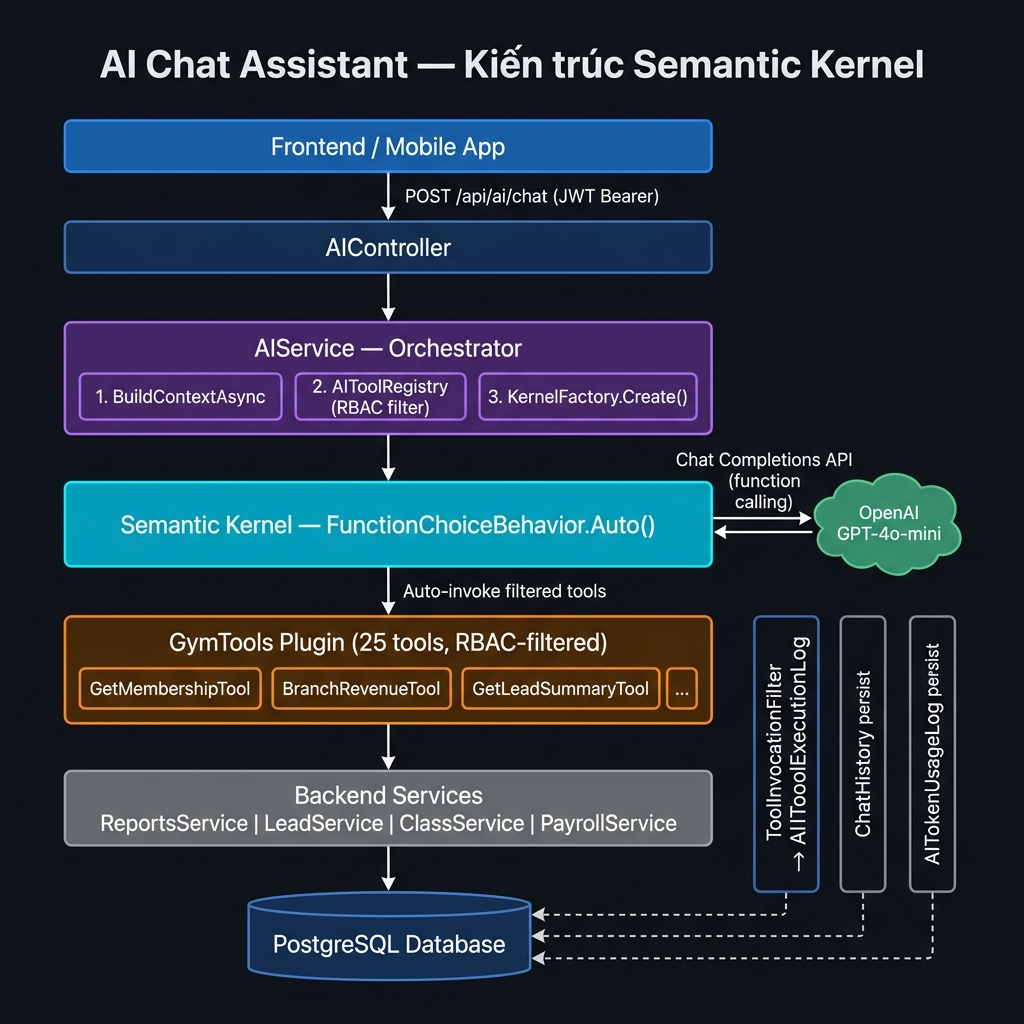
\includegraphics[width=0.92\linewidth]{ai_architecture.png}
    \caption{Kiến trúc tổng quan AI Chat Assistant với Semantic Kernel}
    \label{fig:ai-architecture}
\end{figure}

Luồng xử lý một yêu cầu chat:

\begin{enumerate}
    \item \textbf{Xác thực \& phân quyền}: \texttt{AIController} nhận request, xác minh JWT token, trích xuất \texttt{userId}.

    \item \textbf{Xây dựng ngữ cảnh}: \texttt{AIService.BuildContextAsync()} tra cứu \texttt{Role} và \texttt{StaffPosition} từ ASP.NET Identity và cơ sở dữ liệu.

    \item \textbf{Lọc công cụ RBAC}: \texttt{AIToolRegistry.GetAvailableTools(ctx)} lọc 25 tools theo Role và StaffPosition --- LLM \textit{không biết} sự tồn tại của các tools nằm ngoài phạm vi quyền hạn của người dùng.

    \item \textbf{Khởi tạo SK Kernel}: \texttt{KernelFactory.Create()} tạo Kernel với connector OpenAI/Ollama. \texttt{SkToolHelper.WrapAsTool()} chuyển đổi từng \texttt{IAITool} thành \texttt{KernelFunction} thông qua closure pattern.

    \item \textbf{Gọi LLM tự động}: \texttt{IChatCompletionService.GetChatMessageContentAsync()} với \texttt{FunctionChoiceBehavior.Auto()} --- Semantic Kernel tự điều phối toàn bộ vòng lặp LLM $\to$ tool $\to$ LLM cho đến khi có câu trả lời cuối.

    \item \textbf{Kiểm tra \& ghi log}: \texttt{ToolInvocationFilter} (triển khai \texttt{IFunctionInvocationFilter} của SK) chặn mỗi lần tool được gọi, ghi \texttt{AIToolExecutionLog} bao gồm tên tool, thời gian thực thi, trạng thái.

    \item \textbf{Lưu trữ}: Lưu lịch sử hội thoại vào \texttt{ChatHistories}, token tiêu thụ vào \texttt{AITokenUsageLogs}, kế hoạch tập luyện vào \texttt{AIRecommendations}.
\end{enumerate}

% ---- Canonical Tool Layer ----
\subsubsection{Lớp Công cụ Chuẩn (Canonical Tool Layer)}

Hệ thống định nghĩa interface \texttt{IAITool} thống nhất cho tất cả 25 công cụ, tổ chức theo domain nghiệp vụ:

\begin{table}[H]
\centering
\renewcommand{\arraystretch}{1.35}
\begin{tabular}{|c|c|c|}
\hline
\textbf{Domain} & \textbf{Số lượng tools} & \textbf{Nhóm người dùng} \\
\hline
Membership & 2 & Member \\
\hline
Booking & 5 & Member, Staff \\
\hline
Attendance & 3 & Member, Staff \\
\hline
Training & 3 & Member, Staff (PT/HeadPT) \\
\hline
Lead/Sales & 3 & Staff (Sales/BranchAdmin), GymOwner, SuperAdmin \\
\hline
Analytics & 3 & Staff, GymOwner, SuperAdmin \\
\hline
Revenue & 3 & Staff (BranchAdmin), GymOwner, SuperAdmin \\
\hline
Payroll & 2 & Staff (BranchAdmin), GymOwner, SuperAdmin \\
\hline
Contract & 1 & Staff, GymOwner, SuperAdmin \\
\hline
\textbf{Tổng} & \textbf{25} & --- \\
\hline
\end{tabular}
\caption{Phân bổ công cụ AI theo domain nghiệp vụ}
\label{tab:ai-tools}
\end{table}

Mỗi tool triển khai 5 thuộc tính:

\begin{itemize}
    \item \texttt{Name}: tên snake\_case duy nhất, LLM dùng để gọi tool.
    \item \texttt{Description}: mô tả ngữ nghĩa giúp LLM quyết định khi nào nên dùng tool.
    \item \texttt{InputSchema}: JSON Schema mô tả tham số đầu vào.
    \item \texttt{AllowedRoles}: danh sách ASP.NET Identity roles được phép (\texttt{Member}, \texttt{Staff}, \texttt{GymOwner}, \texttt{SuperAdmin}).
    \item \texttt{AllowedStaffPositions}: vị trí nghiệp vụ cụ thể trong Staff (\texttt{Sales}, \texttt{PT}, \texttt{HeadPT}, \texttt{Receptionist}, \texttt{BranchAdmin}).
\end{itemize}

% ---- RBAC ----
\subsubsection{Mô hình Phân quyền (RBAC)}

Hệ thống áp dụng hai lớp kiểm soát truy cập độc lập:

\begin{enumerate}
    \item \textbf{Lớp Role}: lọc theo \texttt{AllowedRoles} --- Member không bao giờ nhận \textit{get\_branch\_revenue} hay \textit{get\_payroll\_overview}.
    \item \textbf{Lớp StaffPosition}: với caller là Staff, tiếp tục lọc theo \texttt{AllowedStaffPositions} --- nhân viên Sales không nhận tool dành cho PT.
\end{enumerate}

Kết quả: LLM \textbf{chỉ biết} các tools nằm trong phạm vi quyền hạn của người dùng hiện tại. Đây là cơ chế bảo mật theo thiết kế (\textit{Security by Design}), không phụ thuộc vào validation thủ công.

\begin{table}[H]
\centering
\renewcommand{\arraystretch}{1.3}
\small
\begin{tabular}{|l|c|c|c|c|c|c|}
\hline
\textbf{Tool (ví dụ)} & \textbf{Member} & \textbf{Sales} & \textbf{PT} & \textbf{BranchAdmin} & \textbf{GymOwner} & \textbf{SuperAdmin} \\
\hline
get\_membership\_info    & \checkmark & & & & & \\
\hline
generate\_fitness\_plan  & \checkmark & & & & & \\
\hline
get\_lead\_summary       & & \checkmark & & \checkmark & \checkmark & \checkmark \\
\hline
get\_my\_teaching\_schedule & & & \checkmark & & & \\
\hline
get\_branch\_revenue     & & & & \checkmark & \checkmark & \checkmark \\
\hline
get\_payroll\_overview   & & & & & \checkmark & \checkmark \\
\hline
get\_system\_dashboard   & & & & & \checkmark & \checkmark \\
\hline
\end{tabular}
\caption{Ma trận phân quyền công cụ AI (trích từ 25 tools)}
\label{tab:ai-rbac}
\end{table}

% ---- Hybrid Wrapper Pattern ----
\subsubsection{Hybrid Wrapper Pattern}

Để tích hợp \texttt{IAITool} với Semantic Kernel mà không thay đổi logic nghiệp vụ, hệ thống sử dụng \textbf{Hybrid Wrapper Pattern}: lớp \texttt{SkToolHelper} chuyển đổi từng \texttt{IAITool} thành \texttt{KernelFunction} thông qua \texttt{KernelFunctionFactory.CreateFromMethod()}.

\begin{itemize}
    \item \texttt{ToolExecutionContext} (userId, role, branchId) được truyền qua \textit{closure} --- không lộ vào pipeline của SK.
    \item \texttt{KernelArguments} từ SK được serialize sang \texttt{JsonElement} để gọi \texttt{IAITool.ExecuteAsync()} --- 25 tools \textbf{không thay đổi một dòng code nào}.
    \item JSON Schema trong \texttt{InputSchema} được parse thành \texttt{KernelParameterMetadata} giúp SK mô tả đúng tham số với OpenAI.
\end{itemize}

% ---- Sequence Diagram ----
\subsubsection{Luồng xử lý yêu cầu}

Hình~\ref{fig:ai-sequence} mô tả luồng xử lý khi hội viên gửi câu hỏi yêu cầu tra cứu dữ liệu thực tế.

\begin{figure}[H]
    \centering
    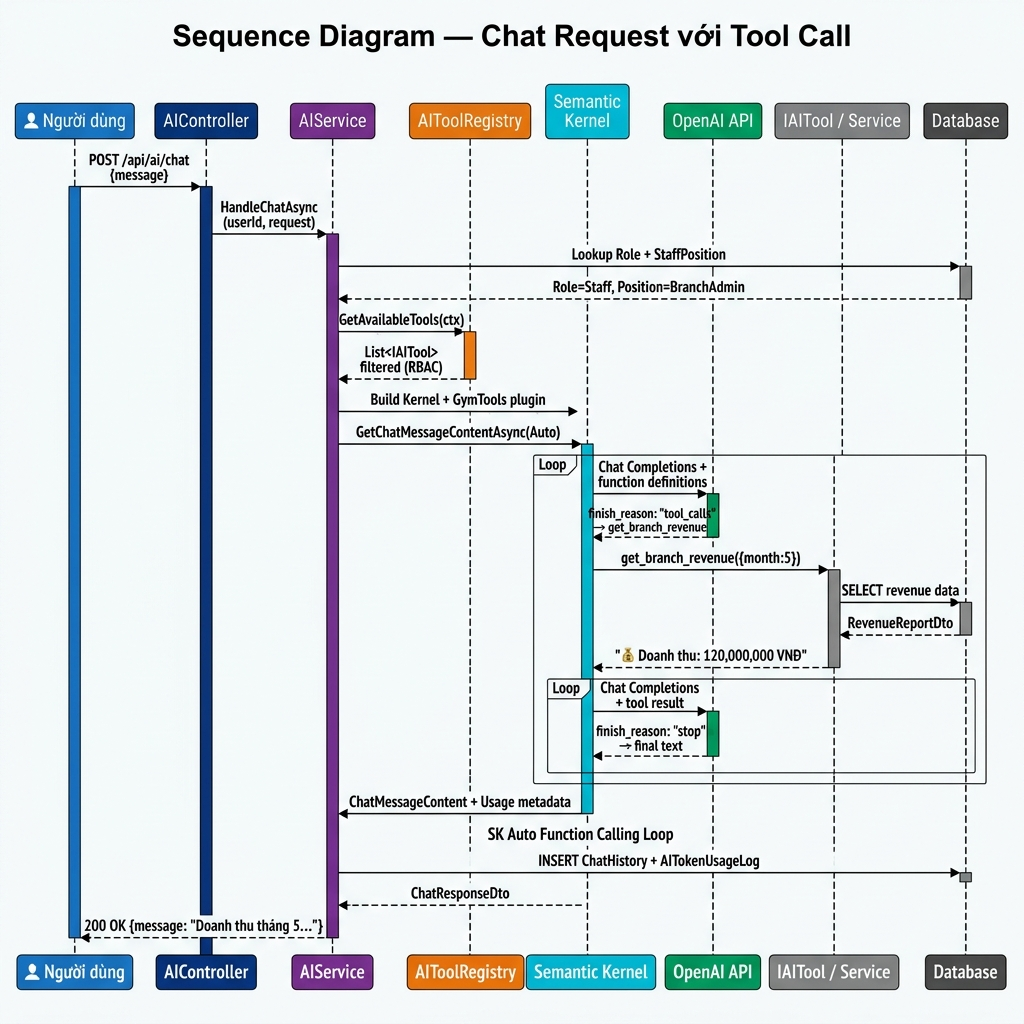
\includegraphics[width=1.0\linewidth]{ai_sequence.png}
    \caption{Sequence diagram: xử lý yêu cầu chat có tool call}
    \label{fig:ai-sequence}
\end{figure}

Điểm khác biệt so với cách tiếp cận thông thường: Semantic Kernel tự động quản lý vòng lặp ``LLM gọi tool --- nhận kết quả --- tiếp tục hội thoại'' thông qua \texttt{FunctionChoiceBehavior.Auto()}, thay vì lập trình thủ công từng bước.

% ---- Cơ sở dữ liệu ----
\subsubsection{Thiết kế Cơ sở dữ liệu}

Module AI bổ sung 4 bảng dữ liệu:

\begin{table}[H]
\centering
\renewcommand{\arraystretch}{1.4}
\begin{tabular}{|l|l|l|}
\hline
\textbf{Bảng} & \textbf{Mục đích} & \textbf{Dữ liệu chính} \\
\hline
\texttt{ChatHistories} & Lưu lịch sử hội thoại & UserId, Role, Message, CreatedAt \\
\hline
\texttt{AIRecommendations} & Kế hoạch tập luyện do AI tạo & WorkoutPlan, NutritionAdvice, Goal \\
\hline
\texttt{AIContextCaches} & Cache hồ sơ hội viên (TTL 6h) & CachedContext, UpdatedAt \\
\hline
\texttt{AIToolExecutionLogs} & Audit trail mỗi lần tool được gọi & ToolName, DurationMs, Success \\
\hline
\texttt{AITokenUsageLogs} & Theo dõi token tiêu thụ & PromptTokens, CompletionTokens, Model \\
\hline
\end{tabular}
\caption{Các bảng dữ liệu của AI Module}
\label{tab:ai-db}
\end{table}

Bảng \texttt{AITokenUsageLogs} cho phép giám sát chi phí vận hành API theo thời gian thực thông qua endpoint \texttt{GET /api/ai/usage} (chỉ SuperAdmin/GymOwner), trả về tổng token tiêu thụ và chi phí ước tính (USD) theo từng vai trò người dùng.

% ---- API Endpoints ----
\subsubsection{Các API Endpoints}

\begin{table}[H]
\centering
\renewcommand{\arraystretch}{1.35}
\begin{tabular}{|l|l|l|l|}
\hline
\textbf{Method} & \textbf{Endpoint} & \textbf{Phân quyền} & \textbf{Mô tả} \\
\hline
POST & \texttt{/api/ai/chat} & Mọi role & Chat với AI \\
\hline
GET  & \texttt{/api/ai/history} & Mọi role & Lịch sử hội thoại \\
\hline
GET  & \texttt{/api/ai/tools} & Mọi role & Danh sách tools (theo RBAC) \\
\hline
GET  & \texttt{/api/ai/recommendations} & Member & Kế hoạch tập luyện đã lưu \\
\hline
GET  & \texttt{/api/ai/usage} & SuperAdmin, GymOwner & Thống kê token \& chi phí \\
\hline
\end{tabular}
\caption{Danh sách API endpoints của AI Module}
\label{tab:ai-endpoints}
\end{table}

% ---- Kết quả ----
\subsubsection{Kết quả đạt được}

\begin{longtable}{|@{\hskip2pt}L{5cm}@{\hskip2pt}|
                  @{\hskip2pt}L{8cm}@{\hskip2pt}|}

\hline
\textbf{Tiêu chí} & \textbf{Kết quả} \\
\hline
\endfirsthead

\hline
\textbf{Tiêu chí} & \textbf{Kết quả} \\
\hline
\endhead

Build Project
& 0 errors, sử dụng Microsoft.SemanticKernel v1.30.0 \\
\hline

Database Migration
& Tạo thành công 5 bảng AI (bao gồm AITokenUsageLogs mới) \\
\hline

Phân quyền RBAC
& 2 lớp độc lập: Role + StaffPosition; LLM không biết tools ngoài phạm vi quyền \\
\hline

Tích hợp Semantic Kernel
& FunctionChoiceBehavior.Auto() tự động điều phối vòng lặp tool call \\
\hline

Tích hợp OpenAI
& GPT-4o-mini; hỗ trợ parallel function calling \\
\hline

Canonical Tool Layer
& 25 tools phân nhóm theo 9 domain; không thay đổi khi swap LLM provider \\
\hline

Audit Log
& Ghi AIToolExecutionLog qua IFunctionInvocationFilter cho mỗi tool call \\
\hline

Token Tracking
& Lưu AITokenUsageLog mỗi cuộc hội thoại; ước tính chi phí USD \\
\hline

Lịch sử hội thoại
& Lưu và nạp 20 lượt gần nhất theo UserId + Role \\
\hline

Kế hoạch tập luyện
& Sinh và lưu AIRecommendation cho Member \\
\hline

Provider Agnostic
& Chuyển đổi OpenAI $\leftrightarrow$ Ollama qua config, không sửa code \\
\hline

Bảo mật
& Toàn bộ endpoint yêu cầu JWT; RBAC áp dụng trước khi LLM nhận tool list \\
\hline

\caption{Kết quả triển khai AI Chat Assistant}
\label{tab:ai-result}

\end{longtable}

% ---- Định hướng ----
\subsubsection{Định hướng phát triển}

Trong tương lai, module AI Chat có thể được mở rộng theo các hướng:

\begin{itemize}
    \item \textbf{Streaming response}: trả lời theo thời gian thực thay vì chờ toàn bộ phản hồi, cải thiện trải nghiệm người dùng.

    \item \textbf{Tích hợp Body Metrics}: BMI, cân nặng, body fat percentage vào ngữ cảnh hội viên để cá nhân hóa kế hoạch tập.

    \item \textbf{Multi-turn tool chaining}: các tool phức tạp có thể gọi lẫn nhau theo chuỗi (ví dụ: tra cứu hợp đồng $\to$ tính doanh thu $\to$ so sánh cùng kỳ).

    \item \textbf{Fine-tuned model}: huấn luyện mô hình riêng cho lĩnh vực fitness gym, giảm chi phí và tăng độ chính xác.

    \item \textbf{Cost budget per user}: giới hạn token tiêu thụ theo role (ví dụ: Member tối đa 50.000 tokens/tháng) sử dụng dữ liệu từ \texttt{AITokenUsageLogs}.

    \item \textbf{Dashboard AI analytics}: trực quan hóa hành vi sử dụng, tools phổ biến nhất theo role, xu hướng câu hỏi theo thời gian.
\end{itemize}
